\documentclass[a4paper, 11pt]{article}
\usepackage[utf8]{inputenc}
\usepackage{polski}
\usepackage[polish]{babel}
\usepackage{geometry}
%\usepackage{fontspec}
\geometry{margin=3cm}
\usepackage{graphicx}
\usepackage{enumitem}

\title{Opis zadania projektowego}
\author{Tomasz Bartos, Jakub Dymon, Wiktor Gerstenstein}
%dopisać numery indeksów
\date{16 marca 2016}

\begin{document}
\maketitle
\section{Temat i cel projektu}
Temat: "Internetowy sklep elektroniczny oparty o relacyjną bazę danych"\\
Cel projektu: projekt oraz implementacja aplikacji webowej imitującej sklep internetowy zarówno od strony klienta jak i sprzedawcy
\section{Opis działania i funkcje systemu}
System będzie pozwalał sprzedawcy na dodawanie towarów do sklepu, wystawianie ich do sprzedaży, kontrolę ilości towaru dostępnej na magazynie oraz generowanie prostych raportów na temat sprzedaży, natomiast kupującemu możliwość wyszukiwania towaru, jego zakupu i listowania dokonanych zakupów oraz statusu zamówienia.\\
Aplikacja będzie dostępna w formie strony internetowej umieszczonej na serwerze i dostępnej po zalogowaniu. Będzie istniała możliwość założenia konta w dwóch wariantach - handlowca i klienta - i zależnie od rodzaju konta będzie użytkownikowi udostępniana określona wersja serwisu.
\section{Założenia architektoniczne przyjęte podczas realizacji systemu}
System będzie realizowany w oparciu o relacyjną bazę danych MySQL oraz interfejs dostępowy utworzony w języku PHP. Operacje dostępowe oraz przetwarzanie danych będą się odbywać po stronie bazy danych, natomiast dla klienta udostępnione zostanie graficzne środowisko dostępowe umożliwiające wydawanie żądanych zapytań. Klient będzie miał możliwość sprawdzenia wybranych zawartości tabel, modyfikacji danych oraz ich usuwania. Wykonywanie poleceń w systemie bazodanowym nie będzie wymagało od użytkownika znajomości języka SQL.
\section{Wykorzystywane technologie, narzędzia projektowania oraz implementacji systemu}
Technologie:
\begin{itemize}
	\item PHP 7.0
	\item MySQL 5.7.10
	\item HTML 5
	\item CSS 3
	\item LaTeX (dokumentacja)
\end{itemize}
Narzędzia projektowania:
\begin{itemize}
	\item MySQL 5.7.11
\end{itemize}
Narzędzia implementacji systemu:
\begin{itemize}
	\item GitHub Desktop 3.0.15
	\item NetBeans IDE 8.1
	\item XAMPP 5.6.19
\end{itemize}
\section{Schemat komunikacji, struktura systemu}
\begin{figure}[h]
	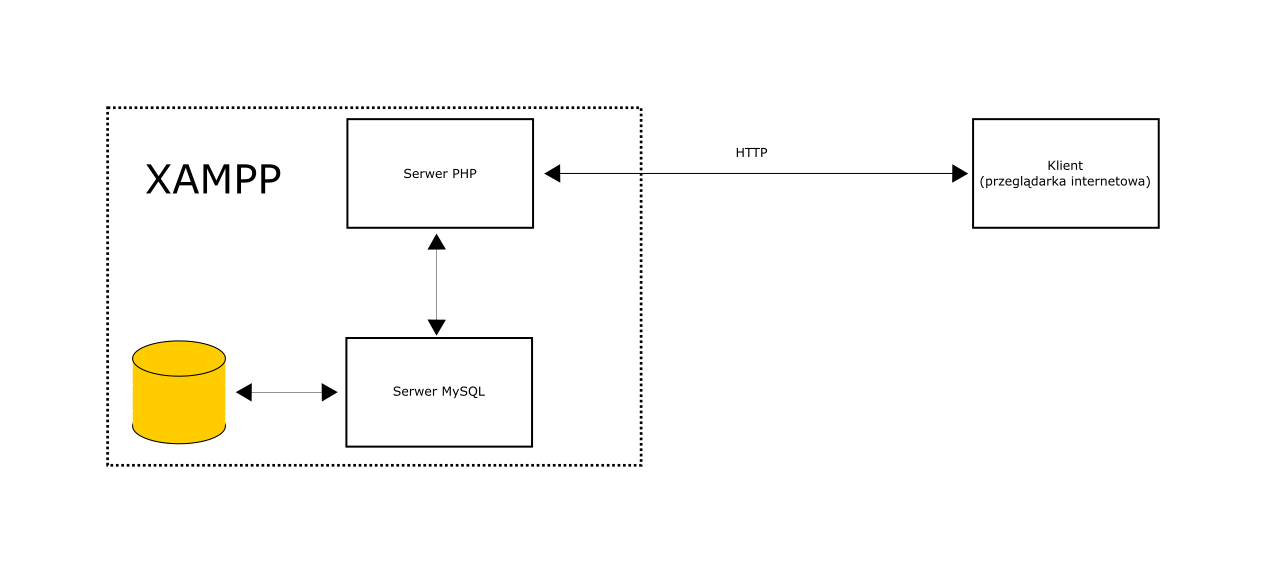
\includegraphics[width=15cm]{schemat.png}
\end{figure}
\section{Literatura}
\begin{enumerate}[label={[\arabic*]}]
	\item Kierzkowski A., \textit{PHP5. Tworzenie stron WWW}, Helion, Gliwice 2006
	\item http://www.kurshtml.edu.pl/
	\item http://php.net/
	\item http://www.w3schools.com/html/default.asp
	\item http://www.w3schools.com/sql/default.asp
\end{enumerate}
\end{document}